%%%%%%%%%%%%%%%%%%%%%%%%%%%%%%%%%%%%%%%%%%%%%%%%%%%%%%%%%%%%%%%%%%%%%
%                                                                   %
%	CHAPTER THREE, SOFTWARE AND API                                   %
%                                                                   %
%%%%%%%%%%%%%%%%%%%%%%%%%%%%%%%%%%%%%%%%%%%%%%%%%%%%%%%%%%%%%%%%%%%%%

\chapter{Software in HPC}

\section{Introduction}
After presenting the rules of HPC and the hardware that compose the cluster, we introduce the most famous ways to target those architectures and supercomputers. 
Several options are present in the language, the multi-processing API, the distribution and the accelerators code. 
This chapter details the most important software options for HPC programming and include the choices we made for our applications.

Then it presents the software used to benchmark the supercomputers. 
We present here the most famous, the TOP500, GRAPH500 and GREEN500 to give their advantages and weaknesses. 

%\todo{Parler des pitfalls, load balancing, concurrence, ... NON dans la partie 2 avant la metrique mise en place ? }

\section{Parallel and distributed programming Models}

\subsection{Parallel Random Access Machine}
The PRAM model is charactrized as follow: 
\begin{itemize}
  \item[-] blahblah
  \item[-] Register and local memory per processors
\end{itemize}

\subsection{Distributed Random Access Machine}

\subsubsection{H-PRAM}

\subsubsection{Bulk Synchronous Parallelism }

\subsection{Hybridation}

\section{Software/API}
In this section we present the main runtime, API and frameworks use in HPC and in this study in particular. 
The considered language will be C/C++, the most present in HPC world along with Fortran. 

\subsection{Shared memory programming}
On the supercomputers nodes we find one or several processors that access to UMA or NUMA memory. 
Several API and language provide tools to target and handle concurrency and data sharing in this context. 
The two main ones are PThreads and OpenMP for multi-core processors. 
We can also cite Cilk++ or TBB from Intel.

\subsubsection{PThreads}
The Portable Operating System Interface (POSIX) threads API is an execution model based on threading interfaces. 
It is developed by the IEEE Computer Society. 
It allows the user to define threads that will execute concurrently on the processor resources using shared/private memory.
PThreads is the low level handling of threads and the user need to handle concurrency with semaphores, conditions variables and synchronization "by hand".
This makes the PThreads hard to use in complex applications and used only for very fine-grained control over the threads management. 

\subsubsection{OpenMP}
Open Multi-Processing, OpenMP\footnote{http://www.openmp.org}~\cite{chapman2008using,supinski2017scaling}, is an API for multi-processing shared memory like UMA and CC-NUMA.
It is available in C/C++ and Fortran.
The user is provided with pragmas and functions to declare parallel loop and regions in the code. 
In this model the main thread, the first one before forks, command the fork-join operations. 

The last versions of OpenMP also allow the user to target accelerators. 
During compilation the user specify on which processor or accelerator the code will be executed in parallel. 

\subsection{Distributed programming}
In the cluster once the code have been developed locally and using the multiple cores available, the new step is to distribute it all over the nodes of the cluster. 
This step requires the processes to access NoRMA memory from a node to another. 
Several runtime are possible for this purpose and concerning our study. 
We should also cite HPX, the c++ standard distribution library, or AMPI for Adaptive MPI, Multi-Processor Computing (MPC) from CEA, etc.

\subsubsection{MPI}
The Message Passing Interface, MPI, is the most famous runtime for distributed computing~\cite{gropp2014using,gropp2015using}.
Several implementations exists from Intel MPI\footnote{https://software.intel.com/en-us/intel-mpi-library} (IMPI), MVAPICH\footnote{http://mvapich.cse.ohio-state.edu/} by the Ohio State University and OpenMP\footnote{http://www.open-mpi.org} combining several MPI work like Los Alamos MPI (LA-MPI).
Those implementation follow the MPI standards 1.0, 2.0 or the latest, 3.0. 

This runtime provides directs, collectives and asynchronous functions for process(es) to process(es) communication.
A process can be a whole node or one or several cores on a processor.  

Some MPI implementations offer a support for accelerators targeting directly their memory through the network without multiple copies on host memory. 
The data go through one GPU to the other through network and PCIe.
This feature is used in our code in part 2 and 3.

\begin{figure}
\begin{center}
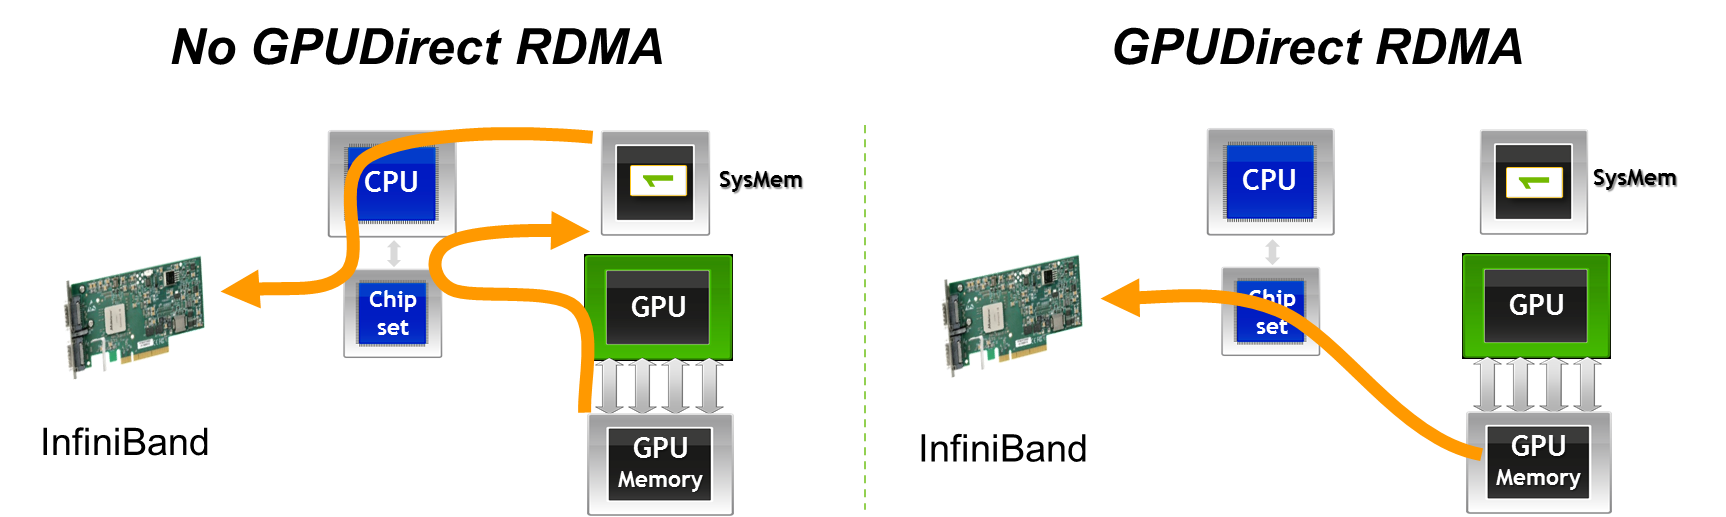
\includegraphics[width=.8\textwidth]{\locpath/figures/chap1/GPUDirectRDMA.png}
\caption{GPUDirect RDMA from NVIDIA Developer Blog, \textit{An Introduction to CUDA-Aware MPI
}}
\label{fig:1_HPC:gpudirect_rdma}
\end{center}
\end{figure}

For NVIDIA this technology is called GPUDirect RDMA and presented on figure~\ref{fig:1_HPC:gpudirect_rdma}. 

In term of development MPI can be very efficient if use carefully. 
Indeed, the collectives communications such as \textit{MPI\_Alltoall}, \textit{MPI\_Allgather}, etc. can be a bottleneck when scaling up to thousands of processes. 
A specific care have to be taken in those implementation with privilege to asynchronous communications to hide computation than synchronous idle CPU time. 

\subsubsection{Charm++}
Charm++\footnote{http://charmplusplus.org/} is an API for distributed programming developed by the University of Illinois Urbana-Champaign.
It is asynchronous messages paradigm driven.
In contrary of runtime like MPI that are synchronous but can handle asynchronous, charm++ is natively asynchronous. 
It is based on \textit{chare object} that can be activated in response to messages from other \textit{chare objects} with triggered actions and callbacks. 
The repartition of data to processors is completely done by the API, the user just have to define correctly the partition and functions of the program. 
Charm++ also provides a GPU manager implementing data movement, asynchronous kernel launch, callbacks, etc.

A perfect example can be the hydrodynamics N-body simulation code Charm++ N-body Gravity Solver, ChaNGa~\cite{jetley2010scaling}, implemented with charm++ and GPU support. 

\subsubsection{Legion}
Legion\footnote{http://legion.stanford.edu/} is a distributed runtime support but Stanford University, Los Alamos National Laboratory (LANL) and NVIDIA. 
This runtime is data-centered targeting distributed heterogeneous architectures. 
Data-centered runtime focuses to keep the data dependency and locality moving the tasks to the data and moving data only if requested. 
In this runtime the user defines data organization, partitions, privileges and coherency. 
Many aspect of the distribution and parallelization are then handle by the runtime itself.

The FleCSI runtime develops at LANL provide a template framework for multi-physics applications and is built on top of Legion. 
We give more details on this project and Legion on part 3.  

\subsection{Accelerators}
In order to target accelerators like GPU, several specific API have been developed. 
At first they were targeted for matrix computation with OpenGL or DirectX through specific devices languages to change the first purpose of the graphic pipeline. 
The GPGPUs arriving forced an evolution and new dedicated language to appear. 

\subsubsection{CUDA}
\label{sec:CUDA}
The Compute Device Unified Architecture is the API develop in C/C++ Fortran by NVIDIA to target its GPGPUs. 
The API provide high and low level functions. 
The driver API allows a fine grain control over the executions.

The CUDA compiler is called NVidia C Compiler, NVCC. 
It converts the device code into Parallel Thread eXecution, PTX, and rely to the C++ host compiler for host code. 
PTX is a pseudo assembly language translated by the GPU in binary code that is then execute. 
As the ISA is simpler than CPU ones and able the user to work directly in assembly for very fine grain optimizations. 

\begin{figure*}[t!]
\centering
\setlength\fboxsep{0pt}
\setlength\fboxrule{0.25pt}
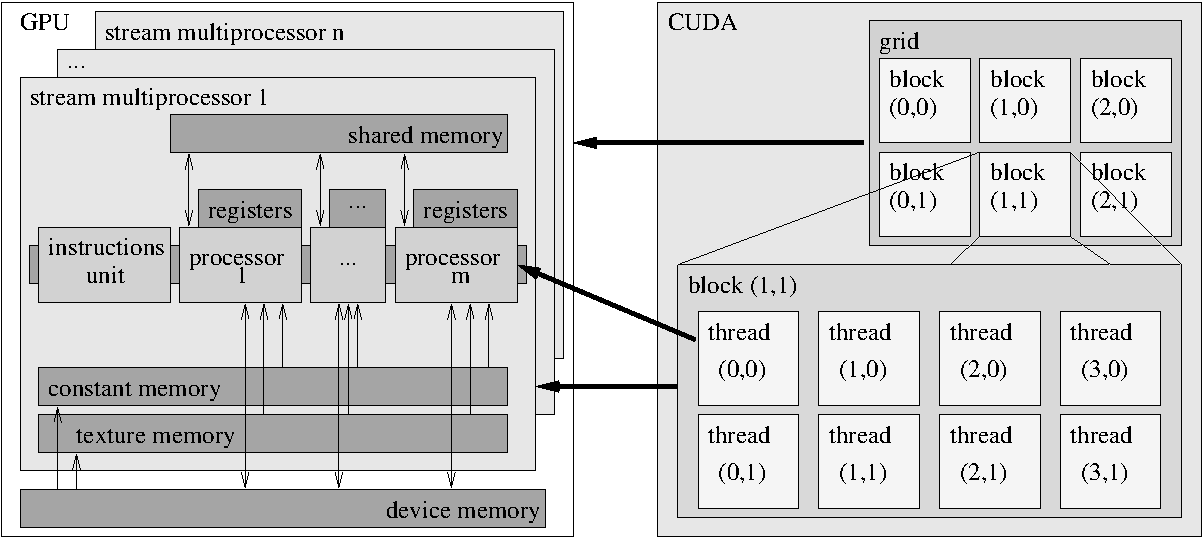
\includegraphics[scale=0.6]{\locpath/figures/chap1/smx}
\caption{NVIDIA GPU and CUDA architecture overview}
 \label{fig:chap1_gpu}
%\vspace{-0.8cm} 
\end{figure*}

As presented in figure~\ref{fig:chap1_gpu}, NVIDIA GPUs include many \emph{Streaming Multiprocessors} (SM), each of which is composed of many \emph{Streaming Processors} (SP). In the Kepler architecture, the SM new generation is called SMX.
%
%In the CUDA programing model~\cite{cuda}, the GPU works as a SIMT co-processor of a conventional CPU. 
Grouped into \emph{blocks}, \textit{threads} execute \emph{kernels} functions synchronously.
Threads within a block can cooperate by sharing data on an SMX and synchronizing their execution to coordinate memory accesses; inside a block, the scheduler organizes \emph{warps} of 32 threads which execute the instructions simultaneously.
The blocks are distributed over the GPU SMXs to be executed independently.

%Memory, bandwidth and streams:
In order to use data in a device kernel, it has to be first created on the CPU, allocated on the GPU and then transferred from the CPU to the GPU; after the kernel execution, the results have to be transferred back from the GPU to the CPU. 
GPUs consist of several memory categories, organized hierarchically and differing by size, bandwidth and latency.   
On the one hand, the device's main memory is relatively large but has a slow access time due to a huge latency. 
On the other hand, each SMX has a small amount of shared memory and L1 cache, accessible by its SPs, with faster access, and registers organized as an SP-local memory. 
SMXs also have a constant memory cache and a texture memory cache.
%, that are linked to the constant and texture memories physically located in the device memory: these are read-only and have faster access time than the rest of the memory categories.
Reaching optimal computing efficiency requires considerable effort while programming.
Most of the global memory latency can then be hidden by the threads scheduler if there is enough computational effort to be executed while waiting for the global memory access to complete. Another way to hide this latency is to use streams to overlap kernel computation and memory load. 

%Threads synchronization:
It is also important to note that branching instructions may break the threads synchronous execution inside a warp and thus affect the program efficiency. 
This is the reason why test-based applications, like combinatorial problems that are inherently irregular, are considered as bad candidates for GPU implementation.\\ 
%This is particularly true with regard to combinatorial problems resolution. 
%Thus we intend to provide a way to regularize their execution, in order to get good acceleration with GPU computation. 

Specific tools have been made for HPC in the NVIDIA GPGPUs. 
\begin{description}[noitemsep,nolistsep]
  \item[Dynamic Parallelism] This feature allow the GPU kernels to run other kernels themselves. This feature 
  \item[Hyper-Q] This technology enable several CPU threads to execute kernels on the same GPU simultaneously. This can help to reduce the synchronization time and idle time of CPU cores for specific applications.
  \item[NVIDIA GPU-Direct] GPUs' memory and CPU ones are different and the Host much push the data on GPU before allowing it to compute. GPU-Direct allows direct transfers from GPU devices through the network. Usually implemented using MPI.  
\end{description}

\subsubsection{OpenCL}
OpenCL is a multi-platform framework targeting a large part of nowadays architectures from processors to GPUs, FPGAs, etc.
A large group of company already provided conform version of the OpenCL standard: IBM, Intel, NVIDIA, AMD, ARM, etc.
This framework allows to produce a single code that can run in all the host or device architectures. 
It is quite similar to NVIDIA CUDA Driver API and based on kernels that are written and can be used in On-line/Off-line compilation meaning Just In Time (JIT) or not. 
The idea of OpenCL is great by rely on the 
Indeed, one may wonder, what is the level of work done by NVIDIA on its own CUDA framework compare to the one done to implement OpenCL standards? 
What is the advantage for NVIDIA GPU to be able to be replace by another component and compare on the same level? 
Those questions are still empty but many tests prove that OpenCL can be as comparable as CUDA but rarely better\cite{karimi2010performance,fang2011comprehensive}. 

In this study most of the code had been developed using CUDA to have the best benefit of the NVIDIA GPUs present in the ROMEO Supercomputer. 
Also the long time partnership of the University of Reims Champagne-Ardenne and NVIDIA since 2003 allows us to exchange directly with the support and NVIDIA developers. 

\subsubsection{OpenACC}
Open ACCelerators is a "user-driven directive-based performance-portable parallel programming model"\footnote{https://www.openacc.org/} developed with Cray, AMD, NVIDIA, etc.
This programming model propose, in a similar way to OpenMP, pragmas to define the loop parallelism and the device behavior. 
As the device memory is separated specific pragmas are use to define the memory movements.
Research works\cite{wienke2012openacc} tend to show that OpenACC performances are good regarding the time spend in the implementation itself compare to fine grain CUDA or OpenCL approaches. 
The little lack of performances can also be explain by the current contribution to companies in the wrapper for their architectures and devices. 

\begin{figure}
\centering 
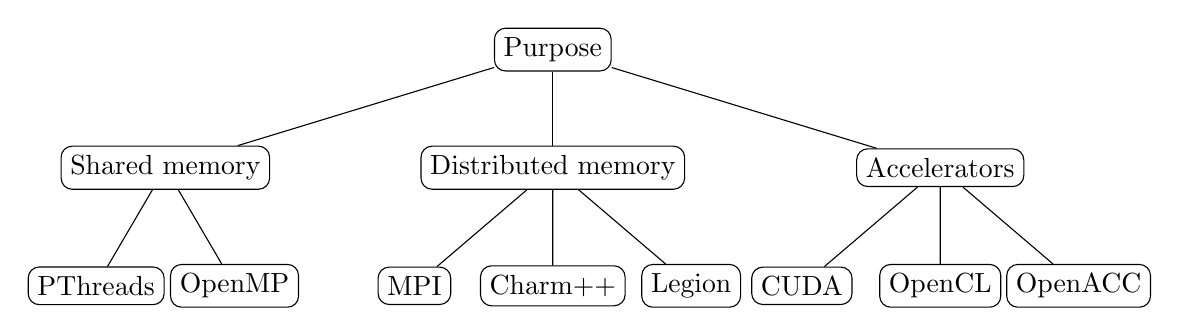
\begin{tikzpicture}[
  every node/.style = {
    level distance=1em,
    shape=rectangle, 
    rounded corners,
    draw, 
    align=center,
    top color=white%, 
   % bottom color=blue!20
  }]]
  \node {Purpose} [sibling distance=14em]
    child { node {Shared memory} [sibling distance=5em]
      child { node {PThreads}}
      child { node {OpenMP}}
    }
    child { node {Distributed memory} [sibling distance=5em]
        child{node {MPI}} 
        child{node {Charm++}}
        child{node {Legion}}
    }
    child { node {Accelerators} [sibling distance=5em]
      child {node  {CUDA}} 
      child { node {OpenCL}}
      child {node {OpenACC}}
    };
\end{tikzpicture}
\caption{Runtimes, libraries, frameworks or APIs}
\label{fig:1_HPC:software}
\end{figure}

The runtime, libraries, frameworks and APIs are summarized in figure~\ref{fig:1_HPC:software} 
They are used in combination. 
The usual one is MPI for distribution, OpenMP and CUDA to target processors and GPUs. 

%\section{Profiling tools}
%\todo{Est-ce interessant? Plus tard? Ne pas en parler?}
%\subsection{Intel suite}
%\subsection{MAQAO}
%\subsection{Allinea/MAP}

\section{Benchmarks}

This section regroup a bunch of the most famous nowadays benchmarks for HPC. 

\subsection{TOP500}
The most famous benchmark is certainly the TOP500\footnote{http://www.top500.org}. 
It gives the ranking of the 500 most powerful, known, supercomputers of the world as its name indicates.
Since 1993 the organization assembles and maintains this list updated twice a year in June and November.

This benchmark is based on the LINPACK\cite{dongarra1994top500} a benchmark introduced by Jack J. Dongarra.
This benchmark rely on solving  dense system of linear equations. 
As specified in this document this benchmark is just one of the tools to define the performance of a supercomputer. 
It reflects "the performance of a dedicated system for solving a dense system of linear equations".
This kind of benchmark is very regular in computation giving high results for FLOPS. 

In 1965 the Intel co-fonder Gordon Moore made an observation\cite{present2000cramming} on the evolution of devices. 
He pointed the fact that the number of transistors in a dense integrated circuit doubles approximately every eighteen months.
This is know as the Moore's law. 
Looking at the last TOP500 figure presented on figure~\ref{fig:intro_top500}, in the introduction of this document, we saw that nowadays machines does not fit in the law anymore. 
This is due to the size of transistor and the energy needed to reach more powerful machines. 
The Moore's law have been sustains by the arrival of many-cores architectures such as GPU or Xeon Phi. 
Tomorrow machines architectures will have to be based on hybrid with more paradigms and tools to take part of massive parallelism.


\subsection{GREEN500}
In conjunction of the TOP500, the GREEN500\footnote{https://www.top500.org/green500/} focus on the energy consumption of supercomputers. 
The scale is based on FLOPS per watts~\cite{feng2007green500}.
Indeed the energy wall is the main limitation for next generation and exascale supercomputers. 
In the last list, November 2017, the TOP3 machines are accelerated with PEZY-SC many-core devices. 
The TOP20 supercomputers are all equipped with many-cores architectures: 5 with PEZY-SC, 14 with NVIDIA P100 and 1 with the Sunway many-core devices. 
This show clearly that the nowadays energy efficient solutions resides in many-core architecture and more than that, hybrid supercomputers. 

\subsection{GRAPH500}
The GRAPH500\footnote{https://www.graph500.org/} benchmark\cite{murphy2010introducing} focus on irregular memory accesses, and communications.
The authors try to find ways to face the futures large-scale large-data problems and data-driven analysis.
This can be see as a complement of the TOP500 for data intensive applications.
The aim is to generate a huge graph to fill all the maximum memory on the machine and then operate either:
\begin{description}
  \item[BFS:] A Breadth-First Search which is an algorithm starting from a root and exploring recursively all the neighbors. 
  This requires a lot of irregular communications and memory accesses. 
  \item[SSSP:] A Single Source Shortest Path which is an algorithm searching the shortest path from one node to the others. 
  Like the BFS it has an irregular behavior but also requires to keep more data during the computation.
\end{description}

This benchmark will be detailed in Part II Chapter II in our benchmark suite. 

\subsection{HPCG}
The High Performance Conjugate Gradient benchmark is a new benchmark created in 2015 and presented for the first time at SuperComputing 15. 
The last list, November 2017 contains 115 supercomputers ranked. 
The list also offer to compare the results of Linpack compared to Conjugate Gradient. 
This benchmark is a first implementation of having both computation and 
communications aspects of HPC. 

\section{Conclusion}
In this chapter we presented the most used software tools for HPC. 
From inside node with shared memory paradigms, accelerators and distributed memory using message passing runtime with asynchronous or synchronous behavior. 

The tools to target accelerators architectures tend to be less architecture dependent with API like OpenMP, OpenCL or OpenACC targeting all the machines architectures. 
Unfortunately the vendor themselves have to be involve to provide the best wrapper for their architecture. 
In the mean time vendor dependent API like CUDA for NVIDIA seems to deliver the best performances.

We show through the different benchmark that hybrid architecture start to have their place even in computation heavy and communication heavy context. 
They are the opportunity to reach exascale supercomputers in horizon 2020.  

